% !TeX spellcheck = en_US
\documentclass[RAIstudentexpose%      style
              ,optBibtex%              bibliography tool
              ,optBibstyleAlphabetic% bibliography style
              ,optEnglish%            language
              %,optTikzExternalize%   compiles faster for large tikz images
              %,optExzellenz%
              ]{RAIlatex}%
%
% Set paths
\graphicspath{{figures/}}%
\addbibresource{source/literature.bib}%
\nocite{*}
%
\begin{document}%

% Titlepage
% ---------

\RAIstudentexposeTitlePageMastersThesis{Monocular 3D Traffic Perception Using HD Maps as an Auxiliary Feature}{Joseph M. Birkner}{03704462}{joseph.birkner@tum.de}{\RAInamesProfKnoll}{\RAIutilsToday}%

\section{\RAIlangGerEng{Aufgabenstellung}{Topic}}

This work is conducted within the scope of the \textbf{Providentia++} project. The project aims to provide cars with Digital Twins in the cloud, facilitating enhanced traffic prediction and micro-routing abilities for safer autonomous driving. Under the Providentia project, Sensor packages, encompassing RGB Cameras, Radar, and Lidar, are installed along major roads and intersections. We are evaluating, which minimal Sensor-suite would be suitable for a wider rollout of the sensing infrastructure under minimum cost. 

The "Digital Twin" data-point of a vehicle consists of multiple components: First and foremost, position $\left(x|y|z\right)$, size $\left(w|h|d\right)$ and orientation ($\theta$) are key variables which define a vehicle's spatial state. Since the RGB camera sensor is the cheapest among the installed package, 3D object detection from 2D video is an important area of research within Providentia.

A working initial approach for monocular 3D detection for Providentia++ was developed by Leon Blumenthal \cite{thesisleon} in the scope of their Bachelor's thesis, using 3D projection of the lower edge of 2D vehicle segments. This approach works very well for vehicles which are moving in straight lines, as the orientation can be fixed to a constant value. However, more work needs to be done for reliable monocular detection when observing traffic scenes with heavily varying vehicle orientations, especially scenes such as complex intersections.

The goal of this work is to improve the orientation estimation of turning vehicles by exploiting clues about their heading from HD maps of the observed road scene. Both map-matching and heading estimation will also benefit from considering the prior trajectory of a vehicle. The trajectory can be obtained by chaining observations of an individual vehicle across multiple video frames, thereby introducing a time component to the observation. Once bounding box estimates between frames are related through vehicle identities, it will also become possible to stabilize predictions about their spatial state via Kalmann Filters, Recurrent Neural Networks or other methods.

\section{\RAIlangGerEng{Lösungsansatz}{Approach}}

\subsection{Architecture}

Considering prior work, we have identified several ways in which we amy incorporate map data into the 3D detection process. Within the taxonomy provided by \cite{survey2022}, we are mainly looking at \textit{Result-based Lifting Methods}. Within such approaches, the detection pipeline is divided into a 2D detection and a 3D lifting stage. The 2D detection stage is facilitated by a 2D instance segmentation model such as YoloV5 or YoloActEdge. The 3D lifting stage can then focus on 3D keypoint estimation for each detected instance, which is a much narrower task than full end-end monocular 3D detection. \par

While there are many recent papers on the topic, we have picked two approaches among recent work which we are going to consider for implementation and further development in this thesis: TrafficNet \cite{trafficnet2021} and UrbanNet \cite{urbannet2021}. For TrafficNet, HD map data could directly be used to seed the initial heading estimate. In the paper, this is currently done by matching the vehicle position to the nearest road boundary detected from sattelite imagery (see \cref{fig:tranet-road-edge}). TrafficNet also provides a very fine-tuned rulebook for smoothing 3D detections for individual vehicles over time. \par

\begin{figure}[htb]%
    \centering
    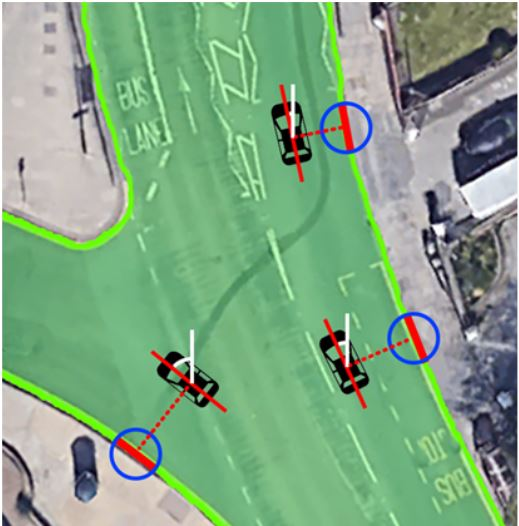
\includegraphics[width=60mm]{angle-estimation}
    \caption{Figure 12 regarding Angle Estimation from Traffic-Net \cite{trafficnet2021}}
    \label{fig:tranet-road-edge}%
\end{figure}%

The drawback of TrafficNet is that the bounding box height and length predictions are based on hard-coded prior assumptions for their detected object categories. This is solved a bit more elegantly in UrbanNet, which employs a convolutional neural network to detect 3D keypoints for vehicles within their 2D image bounding box (check out \cref{fig:keypoints}). See \cref{fig:urbnet} for an overview of the UrbanNet architecture. \par

\begin{figure}[htb]%
    \centering
    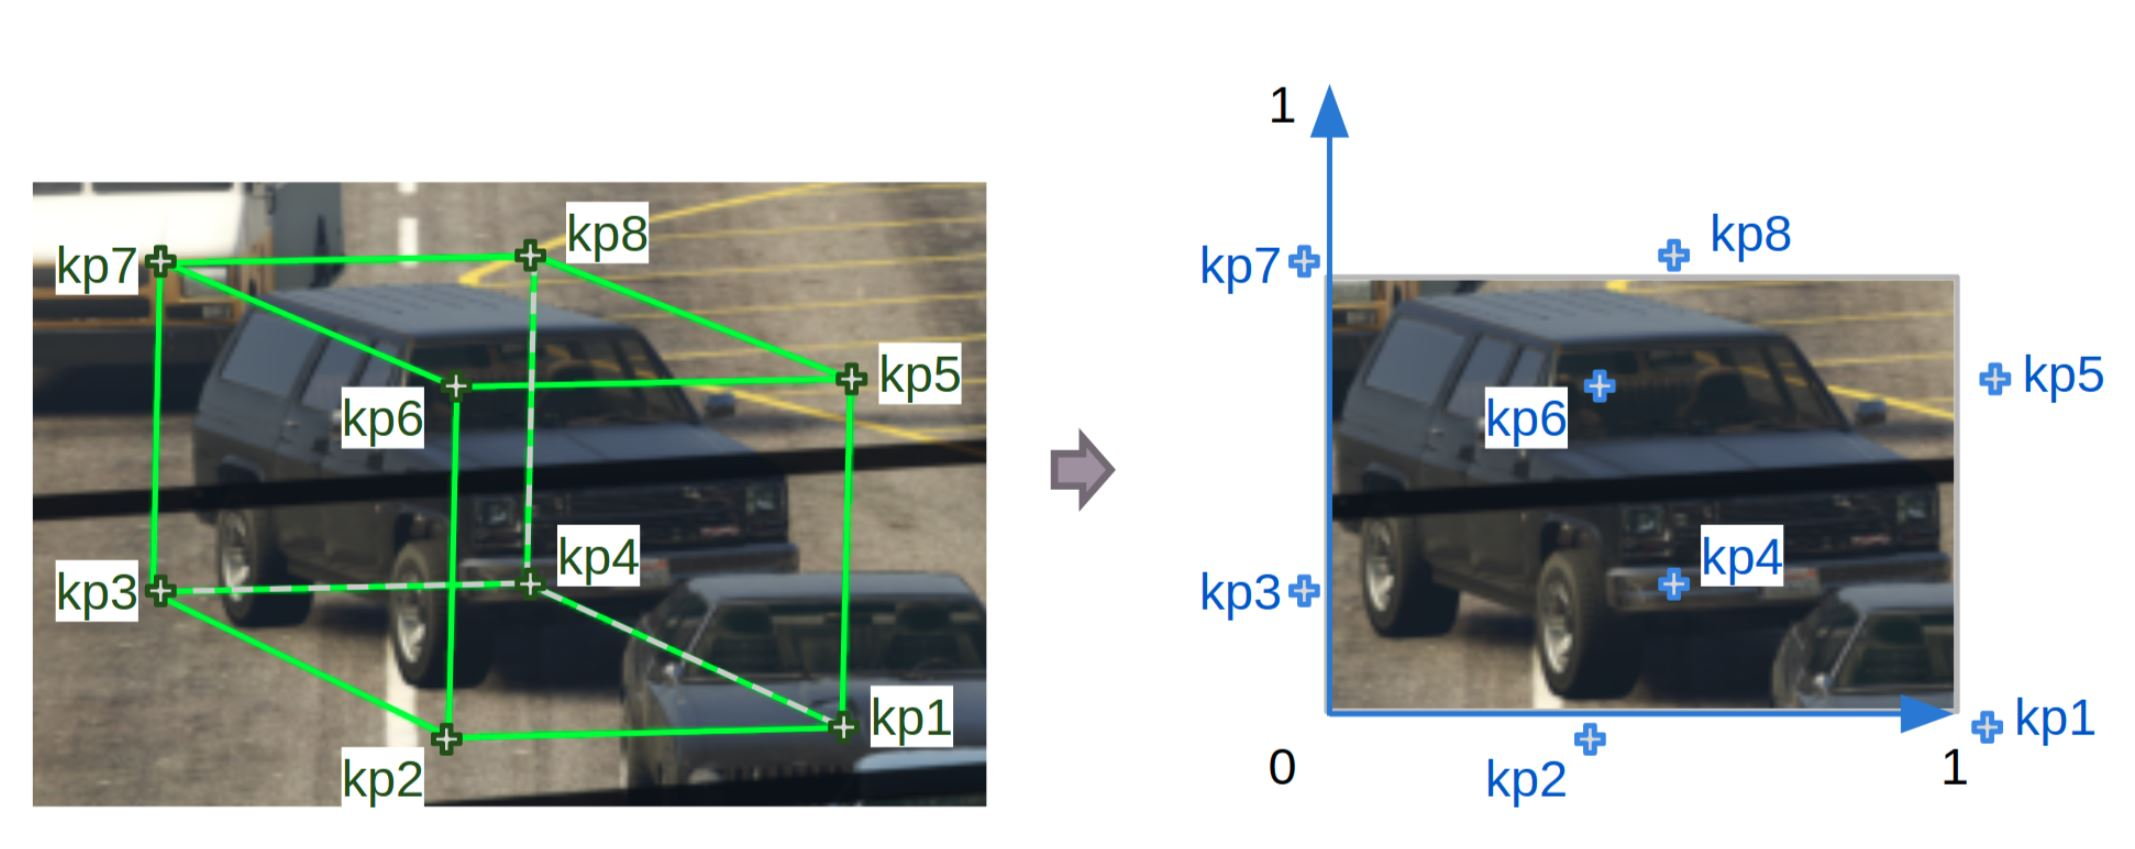
\includegraphics[width=120mm]{keypoints}
    \caption{Figure 4 regarding Keypoint Estimation from UrbanNet \cite{urbannet2021}}
    \label{fig:keypoints}%
\end{figure}%

\begin{figure}[htb]%
    \centering
    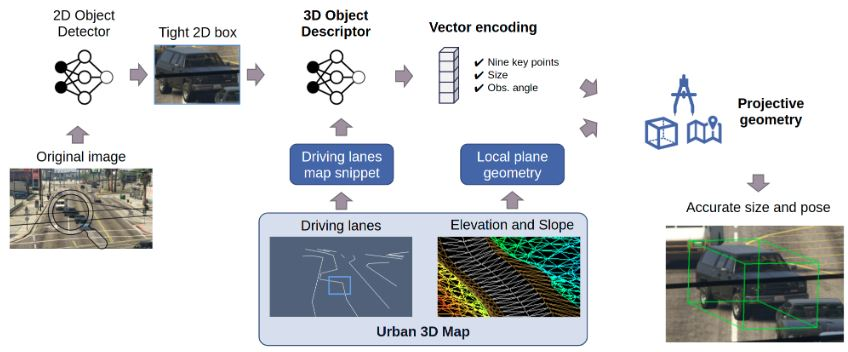
\includegraphics[width=120mm]{urbnet}
    \caption{Figure 2 regarding Architecture from UrbanNet \cite{urbannet2021}}
    \label{fig:urbnet}%
\end{figure}%

For our system design, we are looking to combine the best of these two approaches: Strong temporally informed, map-guided heading estimation, with dynamic neural keypoint extraction. \par

\subsection{Map Format}

We have chosen Lanetlet2 \cite{lanelet22018} as the input map format for our system, as the underlying model is very focused on lanes. This approach is well-suited to inform heading estimation and map-matching of vehicle trajectories. \par

\subsection{Datasets}

Labeled Datasets for the monocular 3D detection task are required for training of supervised machine-learning based components and evaluation of the final system. We are considering to use the following datasets for Training and Evaluation:

\begin{itemize}
\item The Providentia A9 dataset \cite{a92022}
\item The Roadside Perception (ROPE) 3D dataset \cite{rope3d2022}
\item The KITTI dataset \cite{kitti2012}
\item The nuScenes dataset \cite{nuscenes2020}
\end{itemize}

%
\section{\RAIlangGerEng{Arbeitsplan und benötigte Ressourcen}{Work Plan and necessary Resources}}

My work is divided into Research, Development and Evaluation, and Analysis.

\begin{figure*}[!htb]%
    \centering%
    \begin{ganttchart}[%
	y unit chart=.7cm,%
	canvas/.append style={fill=none, draw=black!5, line width=.75pt},%
	hgrid style/.style={draw=black!5, line width=.75pt},%
	vgrid={*1{draw=black!5, line width=.75pt}},%
	title/.style={draw=none, fill=none},%
	title label font=\bfseries\footnotesize,%
	%title label node/.append style={below=5pt},%
	include title in canvas=false,%
	bar height=0.3,%
	bar label font=\mdseries\footnotesize\color{black!70},%
	bar label node/.append style={left=0.2cm},%
	bar/.append style={draw=none, fill=TUMBlue4},%
	group height=0.3,%
	group label node/.append style={left=0.2cm},%
	group label font=\bfseries\small\color{black},%
	group/.append style={draw=none, fill=TUMBlue},%
	]{1}{24}%
	\gantttitle[title label node/.append style={below left=7pt and 10pt}]{Month}{1}%
	\gantttitlelist[title label node/.append style={below left=7pt and 10pt}]{1,...,6}{4} \\%
	\ganttgroup{\textbf{WP1:} Activity A}{1}{5} \\%
	\ganttbar{Activity A11}{1}{3} \\%
	\ganttbar{Activity A12}{2}{5} \\%
	\ganttgroup{\textbf{WP2:} Activity B}{4}{8} \\%
	\ganttbar{Activity A21}{4}{8} \\%
	\ganttgroup{\textbf{WP3:} Activity C}{6}{20} \\%
	\ganttbar{Activity A31}{6}{17} \\%
	\ganttbar{Activity A32}{6}{12} \\%
	\ganttbar{Activity A32}{10}{20} \\%
	\ganttgroup{\textbf{WP4:} Activity D}{18}{22} \\%
	\ganttbar{Activity A41}{18}{20} \\%
	\ganttbar{Activity A42}{18}{22} \\%
	\ganttgroup{\textbf{WP5:} Activity E}{16}{24} \\%
	\ganttbar{Activity A51}{16}{24}%
\end{ganttchart}%

    \caption{Time schedule.}%
\end{figure*}%

% References
\section{\RAIlangGerEng{Literatur}{Literature}}%

\printbibliography[heading=none]%

\end{document}%
